\documentclass[11pt,epsf]{report}
\setlength{\vsize}{297mm}
\setlength{\hsize}{210mm}
\setlength{\textheight}{230mm}
\setlength{\textwidth}{170mm}
%\voffset -2.5cm
\hoffset -2.5cm

\usepackage[latin1]{inputenc}
%\usepackage{latexsym}
%\usepackage{amssymb}
\usepackage[dvips]{graphicx}


\renewcommand\contentsname{Conte\'udo}
\renewcommand\listfigurename{Lista de Figuras}
\renewcommand\listtablename{Lista de Tabelas}
\renewcommand\bibname{Bibliografia}
\renewcommand\indexname{Indice}
\renewcommand\figurename{Figura}
\renewcommand\tablename{Tabela}
\renewcommand\partname{Parte}
\renewcommand\chaptername{Cap�tulo}
\renewcommand\appendixname{Ap\^endice}
\renewcommand\abstractname{Resumo}
\renewcommand\today{\ifcase\month\or
  Janeiro\or Fevereiro\or Mar�o\or Abril\or Maio\or Junho\or
  Julho\or Agosto\or Setembro\or Outubro\or Novembro\or Dezembror\fi
  \space\number\day, \number\year}

\newtheorem{algo}{Algoritmo}
\newcommand\balgo{\begin{algo}}
\newcommand\ealgo{\end{algo}}
\newtheorem{theor}{Teorema}
\newcommand\bth{\begin{theor}}
\newcommand\eth{\end{theor}}
\newcommand\fpreuve {$\Box$ \\}
\newtheorem{assum}{Hip\'otese}
\newcommand\bhyp{\begin{hyp}}
\newcommand\ehyp{\end{hyp}}
\newcommand\fhyp {$\lhd$ \\}
\newtheorem{defin}{Defini\c c\~ao}
\newcommand\bdefi{\begin{defin}}
\newcommand\edefi{\end{defin}}
\newtheorem{lemma}{Lema}
\newcommand\blem{\begin{lemma}}
\newcommand\elem{\end{lemma}}
\newtheorem{propo}{Proposi\c{c}\~{a}o}
\newcommand\bpropo{\begin{propo}}
\newcommand\epropo{\end{propo}}
\newtheorem{propr}{Propriedade}
\newcommand\bpropr{\begin{propr}}
\newcommand\epropr{\end{propr}}
\newtheorem{coroll}{Corol\'ario}
\newcommand\bcor{\begin{coroll}}
\newcommand\ecor{\end{coroll}}
\newtheorem{exemp}{Exemplo}
\newcommand\bex{\begin{exemp}}
\newcommand\eex{\end{exemp}}
\newcommand \fexe {$\diamondsuit$ \\}
\newtheorem{remarq}{Observa\c c\~ao}
\newcommand\brem{\begin{remarq}}
\newcommand\erem{\end{remarq}}
\newcommand\ipar{\hspace*{\parindent}}
\newcommand\epar{\vspace{\baselineskip}}
\newcommand\pdef{\stackrel{\bigtriangleup}{=}}
\newcommand\bdm{\begin{displaymath}}
\newcommand\edm{\end{displaymath}}
\newcommand\barray{\begin{array}}
\newcommand\earray{\end{array}}
\newcommand\beqa{\begin{eqnarray}}
\newcommand\eeqa{\end{eqnarray}}
\newcommand\beqan{\begin{eqnarray*}}
\newcommand\eeqan{\end{eqnarray*}}
\newcommand\beq{\begin{equation}}
\newcommand\eeq{\end{equation}}
\newcommand\bc{\begin{center}}
\newcommand\ec{\end{center}}
\newcommand\bit{\begin{itemize}}
\newcommand\eit{\end{itemize}}
\newcommand\bquo{\begin{quote}}
\newcommand\equo{\end{quote}}
\newcommand\ben{\begin{enumerate}}
\newcommand\een{\end{enumerate}}
\newcommand{\ignore}[1]{\iffalse #1 \fi}
\newcommand\tz{{\cal Z}}
\newcommand\tzi{{\cal Z}^{-1}}


\begin{document}

ENG04035 - Sistemas de Controle I

Prof. Jo�o Manoel e Prof. Romeu



\begin{center}
\Large{{\sf LISTA DE EXERC�CIOS}}

{\bf -  N�o Lienaridades em Sistemas de Controle -}
\end{center}


\begin{enumerate}


\item  Projete um controlador n{\~a}o linear (cancelamento da
n�o-linearidade + controle linear) para cada um dos seguintes {\'\i}tens
abaixo, a partir do sistema da figura 1 abaixo.
\begin{description}
    \item[\hspace{0.8cm}a)] Deseja-se ts $\leq$ 2s.
    \item[\hspace{0.8cm}b)] O mesmo sistema de a) com a n{\~a}o
linearidade vista na figura 2. Neste caso, deseja-se \newline ts
$\leq$ 2s e Mo $<$ 10\%.
    \item[\hspace{0.8cm}c)] Considere agora o sistema da  figura 3.
Deseja-se, neste caso, ts $\leq$ 2s e Mo $<$ 10\%. \\
Observa\c{c}{\~a}o: use
as aproxima\c{c}{\~o}es de Pad{\'e} para fazer o projeto do controlador.
\end{description}

% ********************************************************************
% Figura 1
% ********************************************************************
\begin{figure} [!h]
\begin{center}
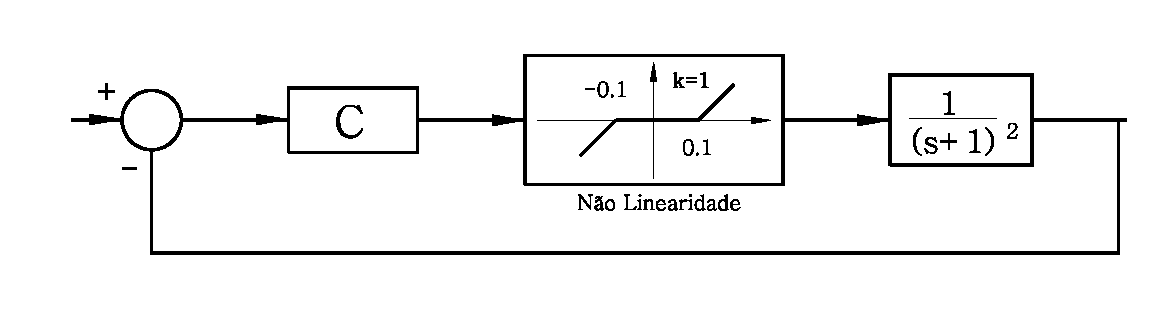
\includegraphics[width=12cm]{NL_1.eps}\end{center}
\caption{Sistema para o item a) da quest{\~a}o 1).} \label{Figura_1}
\end{figure}

% ********************************************************************
% Figura 2
% ********************************************************************
\begin{figure} [!h]
\begin{center}
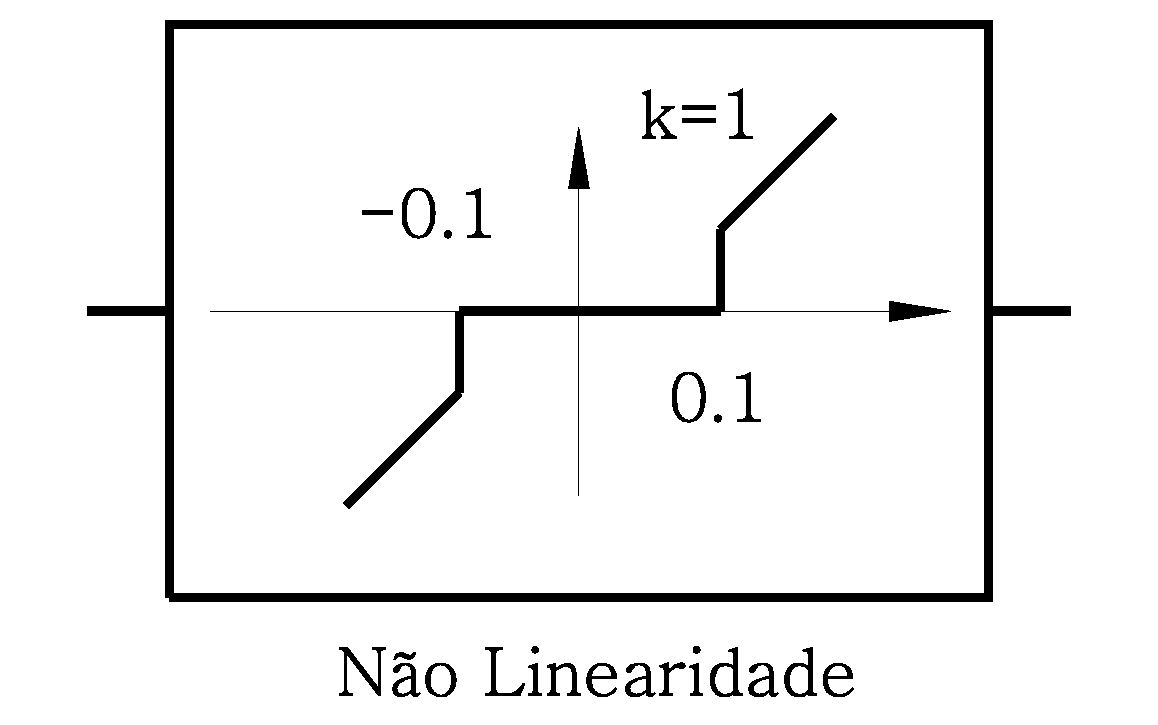
\includegraphics[width=4cm]{NL_2.eps}\end{center}
\caption{N{\~a}o linearidade para o item b) da quest{\~a}o 1).}
\label{Figura_2}
\end{figure}

% ********************************************************************
% Figura 3
% ********************************************************************
\begin{figure} [!h]
\begin{center}
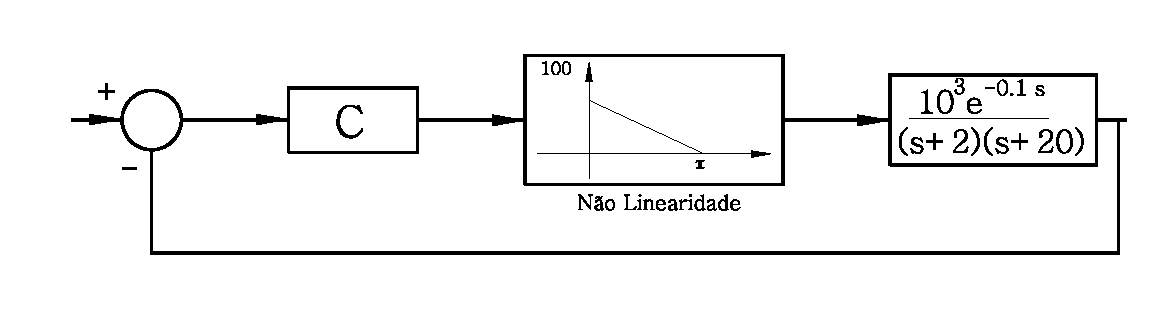
\includegraphics[width=12cm]{NL_3.eps}\end{center}
\caption{Sistema para o item c) da quest{\~a}o 1).} \label{Figura_3}
\end{figure}



\item  Projete um PI para a planta $G(s)=\frac{1}{(s-1)}$
a fim de obter $ts=2s$. Analise por simula\c{c}{\~a}o o efeito de uma
satura\c{c}{\~a}o no controle considerando v{\'a}rios limites de controle
(v{\'a}rios valores de $U_{min}$ e $U_{m\acute{a}x}$ ).

\item  Considerando o sistema da figura 4.
\begin{description}
    \item[\hspace{0.8cm}a)] Analise o comportamento do sistema, esbo�ando 
os sinais $e(t), v(t), u(t)$ e $y(t)$ para uma
refer{\^e}ncia do tipo de salto unit{\'a}rio considerando as seguintes
situa\c{c}{\~o}es:
\begin{enumerate}
    \item $U_{m\acute{a}x}=-U_{min}=0.3$;
    \item $U_{m\acute{a}x}=-U_{min}=0.5$;
    \item $U_{m\acute{a}x}=-U_{min}=0.8$;
    \item $U_{m\acute{a}x}=-U_{min}=1.5$.
\end{enumerate}

Par{\^a}metros do PID na forma s�rie padr�o: $K_p=5.5$, $T_d=1$, $T_i=2$, $\tau=0.01$.

    \item[\hspace{0.8cm}b)] Em todas as situa\c{c}{\~o}es acima o sistema
consegue seguir a refer{\^e}ncia unit{\'a}ria? Justifique.
\end{description}


% ********************************************************************
% Figura 4
% ********************************************************************
\begin{figure} [!h]
\begin{center}
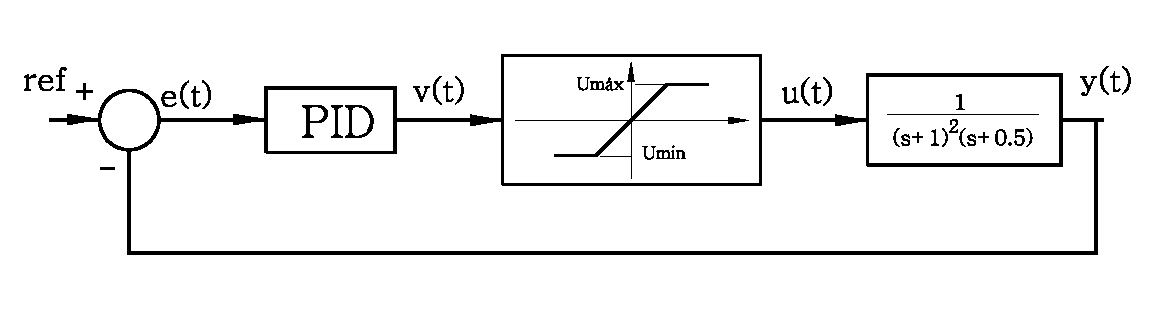
\includegraphics[width=12cm]{NL_4.eps}\end{center}
\caption{Sistema para a quest{\~a}o 3).} \label{Figura_4}
\end{figure}

\end{enumerate}

\end{document}













